\newcommand{\figureElectronicsResistance}[1]{
  \def\lang{\detokenize{#1}}
  \def\langRu{\detokenize{ru}}
  \def\langEn{\detokenize{en}}
  \def\figureCaption{XXX: No translation.}
  \ifx \lang\langRu
  \def\figureCaption{
    Пример ёмкостей, соединённых трубами разных сопротивлений.
  }
  \fi
  \ifx \lang\langEn
  \def\figureCaption{
    An example of two vessels connected with pipes with different resistance to
    the water flow.
  }
  \fi
  \begin{figure}[ht]
    \centering
    \def\offset{6}
    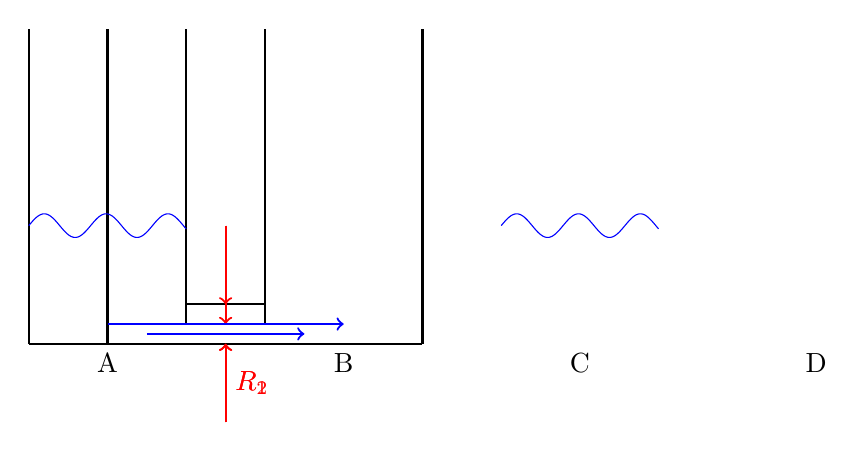
\begin{tikzpicture}[
        declare function={f1(\x) = 0.15 * sin(8.0 * deg(\x));
      }]

      \draw[thick] (0, 0) -- (0, 4);
      \draw[thick] (2, 0.5) -- (2, 4);
      \draw[thick] (0, 0) -- (2, 0);

      \draw[thick] (3, 0.5) -- (3, 4);
      \draw[thick] (5, 0) -- (5, 4);
      \draw[thick] (3, 0) -- (5, 0);

      \draw[thick] (2, 0) -- (3, 0);
      \draw[thick] (2, 0.5) -- (3, 0.5);

      \draw[thick] (\offset, 0) -- (\offset, 4);
      \draw[thick] (\offset + 2, 0.25) -- (\offset + 2, 4);
      \draw[thick] (\offset, 0) -- (\offset + 2, 0);

      \draw[thick] (\offset + 3, 0.25) -- (\offset + 3, 4);
      \draw[thick] (\offset + 5, 0) -- (\offset + 5, 4);
      \draw[thick] (\offset + 3, 0) -- (\offset + 5, 0);

      \draw[thick] (\offset + 2, 0) -- (\offset + 3, 0);
      \draw[thick] (\offset + 2, 0.25) -- (\offset + 3, 0.25);

      \draw[thick, color=red, ->] (2.5, 1.5) -- (2.5, 0.5);
      \draw[thick, color=red, ->] (2.5, -1) -- (2.5, 0);
      \draw[color=red] (2.5, -0.5) node[right] {$R_1$};

      \draw[thick, color=red, ->] (\offset + 2.5, 1.5) -- (\offset + 2.5, 0.25);
      \draw[thick, color=red, ->] (\offset + 2.5, -1) -- (\offset + 2.5, 0);
      \draw[color=red] (\offset + 2.5, -0.5) node[right] {$R_2$};

      \draw[thick, color=blue, ->] (1, 0.25) -- (4, 0.25);

      \draw[thick, color=blue, ->] (\offset + 1.5, 0.125) -- (\offset + 3.5, 0.125);

      \begin{scope}[yshift=1.5cm, color=blue]
        \draw (0, 0) plot[domain=0:2, variable=\x, samples=200, smooth] ({\x}, {f1(\x)});
      \end{scope}

      \begin{scope}[yshift=1.5cm, xshift=6 cm, color=blue]
        \draw (0, 0) plot[domain=0:2, variable=\x, samples=200, smooth] ({\x}, {f1(\x)});
      \end{scope}

      \draw (1, 0) node[below] {A};
      \draw (4, 0) node[below] {B};
      \draw (7, 0) node[below] {C};
      \draw (10, 0) node[below] {D};

    \end{tikzpicture}
    \caption{\figureCaption}
    \label{fig:electronics-resistance-0}
  \end{figure}
}
